\chapter{Magnetic Reconnection in the Jupiter MHD model}

\blfootnote{*Parts of this chapter were published in - Sarkango, Y., Jia, X., \& Toth, G. (2019). Global MHD simulations of the response of Jupiter's magnetosphere and ionosphere to changes in the solar wind and IMF. Journal of Geophysical Research: Space Physics, 124.}

\section{Introduction}
The terrestrial magnetosphere is sensitive to changes in the solar wind and interplanetary magnetic field \cite{Sibeck1991SolarMotion,McPherron2008ResponseWind}. Solar wind dynamic pressure can increase the magnetic stresses in the magnetotail, which increases the frequency of magnetospheric substorms \cite{Kokubun1977TriggeringDiscontinuities,Newell2011SolarTriggering,Newell2016SubstormSpeed}. Dayside magnetic reconnection, which typically occurs due to an anti-parallel (southward) IMF at the magnetopause, creates open field lines on the dayside and facilitates entry of solar wind plasma into the magnetosphere (e.g. \citeNP{Phan2000ExtendedJets}). This can occur during long periods with southward IMF, or as a result of transient features in the solar wind such as coronal mass ejections, whose interiors are comprised of helical magnetic field lines and dense plasma and which travel through the interplanetary medium at supersonic speeds, often creating strong shocks at their travelling front \cite{Webb2012CoronalObservations}. Magnetic reconnection perturbs the terrestrial in various ways, for e.g. by loading the magnetotail and facilitating magnetospheric substorms \cite{Morley2007OnOnsets}, which can lead to auroral phenomena on the nightside \cite{Elphinstone1996WhatSubstorm}, or via geomagnetic storms, which alter the ring current and produce large-scale geomagnetic disturbances \cite{Gonzalez1994WhatStorm}. Magnetic reconnection in the terrestrial system occurs via the opening of flux on the dayside and closure of magnetic flux on the nightside \cite{Dungey1961b}. This cycle of flux circulation (also called the Dungey cycle), also influences plasma flow in the magnetosphere and high-latitude ionospheres, both of which respond to changes in the solar wind dynamic pressure or IMF orientation, which alters the characteristics of magnetic reconnection and thus the Dungey cycle, as discussed in Chapter 1. 

However, considerable debate exists in the community regarding the importance of dayside magnetic reconnection in Jupiter's magnetosphere. Unlike the terrestrial magnetosphere, the strong internal magnetic field and presence of internal sources of plasma lead to a very different magnetospheric configuration.

One argument made against dayside magnetic reconnection highlights the improbable timescales for the Dungey cycle. At Earth, a newly reconnected field line on the dayside, which is frozen-in to the solar wind plasma at its other end, is transported tailward at the solar wind speed of $\sim400$ km/s. Hence, it will take approximately $\sim$300 s or 5 minutes to travel a distance of $\sim20 R_E$ (1 $R_E$ = 6378 km is the radius of the Earth). On the other hand, at Jupiter, a field line opened on the dayside magnetopause would have to travel a distance of $\sim200 R_J$ to reach the magnetotail, which would take  $\sim10$ hours, comparable to the rotation period for Jupiter. Moreover, field lines which have reached the magnetotail may take an even longer time to diffuse towards the equatorial regions where tail reconnection is likely to occur \cite{McComas2007}. 

The two commonly used counter-arguments propose that Dungey cycle timescales may be considerably shorter. This could be possible if the flux circulation occurs in a localized region on the dusk side instead of over the entire magnetosphere like at Earth. Moreover, another hypothesis is that it is not necessary for the field line to fully diffuse toward the equator, as plasmoid release due to the Vasyliunas cycle may also induce reconnection to spread to the open tail lobes \cite{Cowley2008}. 

In-situ observations have shown that magnetic reconnection occurs in the Jovian magnetotail and produces plasmoids. However, single-point measurements cannot help in determining the physical processes which led reconnection to occur. This has been seen via north-south reversals of the magnetic field \cite{Vogt2010a,Vogt2014,Vogt2020MagnetotailObservations} or in the form of bursts of energetic particles with a radial velocity \cite{Woch2002a,Kronberg2007AMagnetosphere,Kronberg2008MassParameters}. The timescales associated with the loading and unloading of the magnetotail (Vasyliunas cycle) has been estimated to be on the order of 2 to 3 days (or 5 to 7 Jovian rotations) \cite{Woch2002a,Vogt2010a}.

Finally, this work is also motivated by observations made by the Hubble Space Telescope of Jupiter's polar regions. The polar UV aurorae are highly dynamic, and vary on timescales much shorter than the main oval. Whether these polar regions of the planet connect to distance regions in the Jovian magnetotail via closed field lines, or to the solar wind via open field lines, remains an open question. 

In this work, we simulate the Jovian magnetosphere using our MHD model to answer the following questions,

\begin{enumerate}
    \item Does magnetic reconnection occur on the dayside magnetopause at Jupiter and create open flux in the magnetosphere?
    \item Does Jupiter have a persistent polar cap of open field lines? 
    \item If so, where and how does flux closure occur in the magnetosphere?
\end{enumerate}

\section{Methodology}
The MHD simulations presented in Chapter 3 were also used in this study. We will primarily be discussing Runs 2 and 4 (see Table \ref{tab:sw-conditions}), which use a Parker-spiral IMF (magnetic field in the $Y$ direction), which is typically expected at Jupiter's orbit. In such situations, the magnetic shear between the IMF and the magnetospheric field at the nose of the magnetopause is 90$^\circ$. The techniques used to analyze the simulation data as described in this section.

\subsection{Identification of the dayside magnetopause surface}
The magnetopause is the surface separating the magnetospheric field from the interplanetary magnetic field. It is a current-carrying discontinuity, and can be identified in MHD simulations as a peak in the current density ($J$). It can also be identified by detecting the increase in density due to the density gradient between the outer magnetosphere and the magnetosheath. In our study, we use magnetic field topology to identify the magnetopause, as this definition is more robust. In our case, the dayside magnetopause is the surface which separates closed magnetic field lines of the magnetosphere from the open field lines in the solar wind. This method is unambiguous on the dayside, but cannot be used for higher latitudes or the magnetotail, which also contain open field lines, but are present inside the magnetosphere. 

A hemispherical surface is created on the dayside at locations $(r=r_i, \theta_i, \phi_i)$ in spherical coordinates. From each point $i$ of the surface, a radial line segment is created to the point $(r=r_o, \theta_i, \phi_i)$, which lies well beyond the dayside bow shock and hence contains solar wind open field lines. A field line is traced from the midpoint of these two locations ($r_m$), and its connectivity is inferred by examining whether its two footprints are traced to the planet (closed) or to the solar wind (open). If the field line is closed, $r_m$ is chosen as the new inner point ($r_i:=r_m$), else $r_m$ is specified as the outer point ($r_o:=r_m$). This binary search algorithm is repeated until $r_o - r_i < 2 R_J$. The resulting midpoint is the location for the magnetopause. The whole process is repeated for each point on the initially hemispherical surface, which produces a new surface for the magnetopause as shown in Figure \ref{fig:reconnection-dayside}. 

\subsection{Classification of a magnetic field line}
Magnetic field lines in the MHD model can only have one of the following properties. Each type is assigned a value in the form of a `status' variable. The field line can be, 

\begin{itemize}
    \item Connected at both ends with the IMF (open field lines or `disconnected', status=0).
    \item Connected to the northern hemisphere of the planet, with the other end connecting to the IMF (open field lines, type N, status=1). 
    \item Connected to the southern hemisphere of the planet, with the other end connecting to the IMF (open field lines, type S, status=2).
    \item Connected at both ends with the planet (closed field lines, status=3)
\end{itemize}

Most field lines in the inner and middle magnetosphere are closed (status=3). The type N and S field lines map to the northern or southern polar cap and are created due to dayside magnetic reconnection.

\subsection{Calculation of the open flux in the polar cap}
In order to estimate the open flux in the polar cap, we must first identify the regions in the northern and southern hemispheres which map to open field lines. This is achieved by creating a spherical surface close to the inner boundary of the MHD simulation domain and tracing field lines at each point of the surface. Points which map to closed field lines are identified, and their corresponding locations at 1 $R_J$ are estimated by using a dipole approximation (due to the existence of a gap between 1 $R_J$ and the inner boundary at 2.5 $R_J$). For an axially aligned dipole field, two points located on the same field line at locations $(r_1, \theta_1)$ and $(r_2, \theta_2)$ are related as,

\begin{equation}
    \frac{r_1}{r_2} = \frac{\sin^2\theta_1}{\sin^2\theta_2}
\end{equation}

The mapping to a sphere at $r=1R_J$ is not necessary to calculate the open flux as the magnetic flux is conserved between the two locations, but it is useful for future comparisons with the ionosphere currents. After the location have been mapped to a sphere with radius $r=1 R_J$, a grid of spherical rectangles is constructed and the magnetic flux through each rectangle corresponding to open field lines is estimated using the dipole field approximation. In this case, for a spherical rectangle of angular widths $\Delta\theta$ and $\Delta\phi$, centered at $(\theta_i, \phi_i)$, the magnetic flux due to a axially aligned dipole field with moment $M$ at a spherical surface with radius $r$ can be calculated analytically - 

\begin{equation}
    \Delta \Phi_i = \iint \mathbf{B} \cdot \mathbf{n}\, dS = \iint B_r dS = \frac{M}{r} \cos(\Delta \phi) \left[ \sin^2 \left( \theta_i + \frac{\Delta\theta}{2}\right) - \sin^2 \left(\theta_i - \frac{\Delta\theta}{2} \right)\right]
\end{equation}

The resulting open flux in the polar cap can be calculated by summing up the contributions due to all regions corresponding to open field lines,

\begin{equation}
    \Phi_\text{open} = \sum \Phi_i\left( \text{status}_i \neq 3 \right)
\end{equation}

\subsection{Calculation of the reconnection rate}
The rate of change of open flux in the polar cap equals the difference in the reconnection rates on the dayside versus that due to Dungey cycle flux closure on the nightside \cite{Milan2007MagneticRates}. If no reconnection is observed on the nightside ($\dot{R}_\text{nightside}=0$), then the dayside reconnection rate can be inferred using the rate of change of the open magnetic flux. 

\begin{equation}
    \frac{d\Phi_\text{open}}{dt} = \dot{R}_\text{dayside} - \dot{R}_\text{nightside}
\end{equation}

\section{Results}

\subsection{Reconnection on the dayside for Parker-spiral IMF}
\begin{figure}
    \centering
    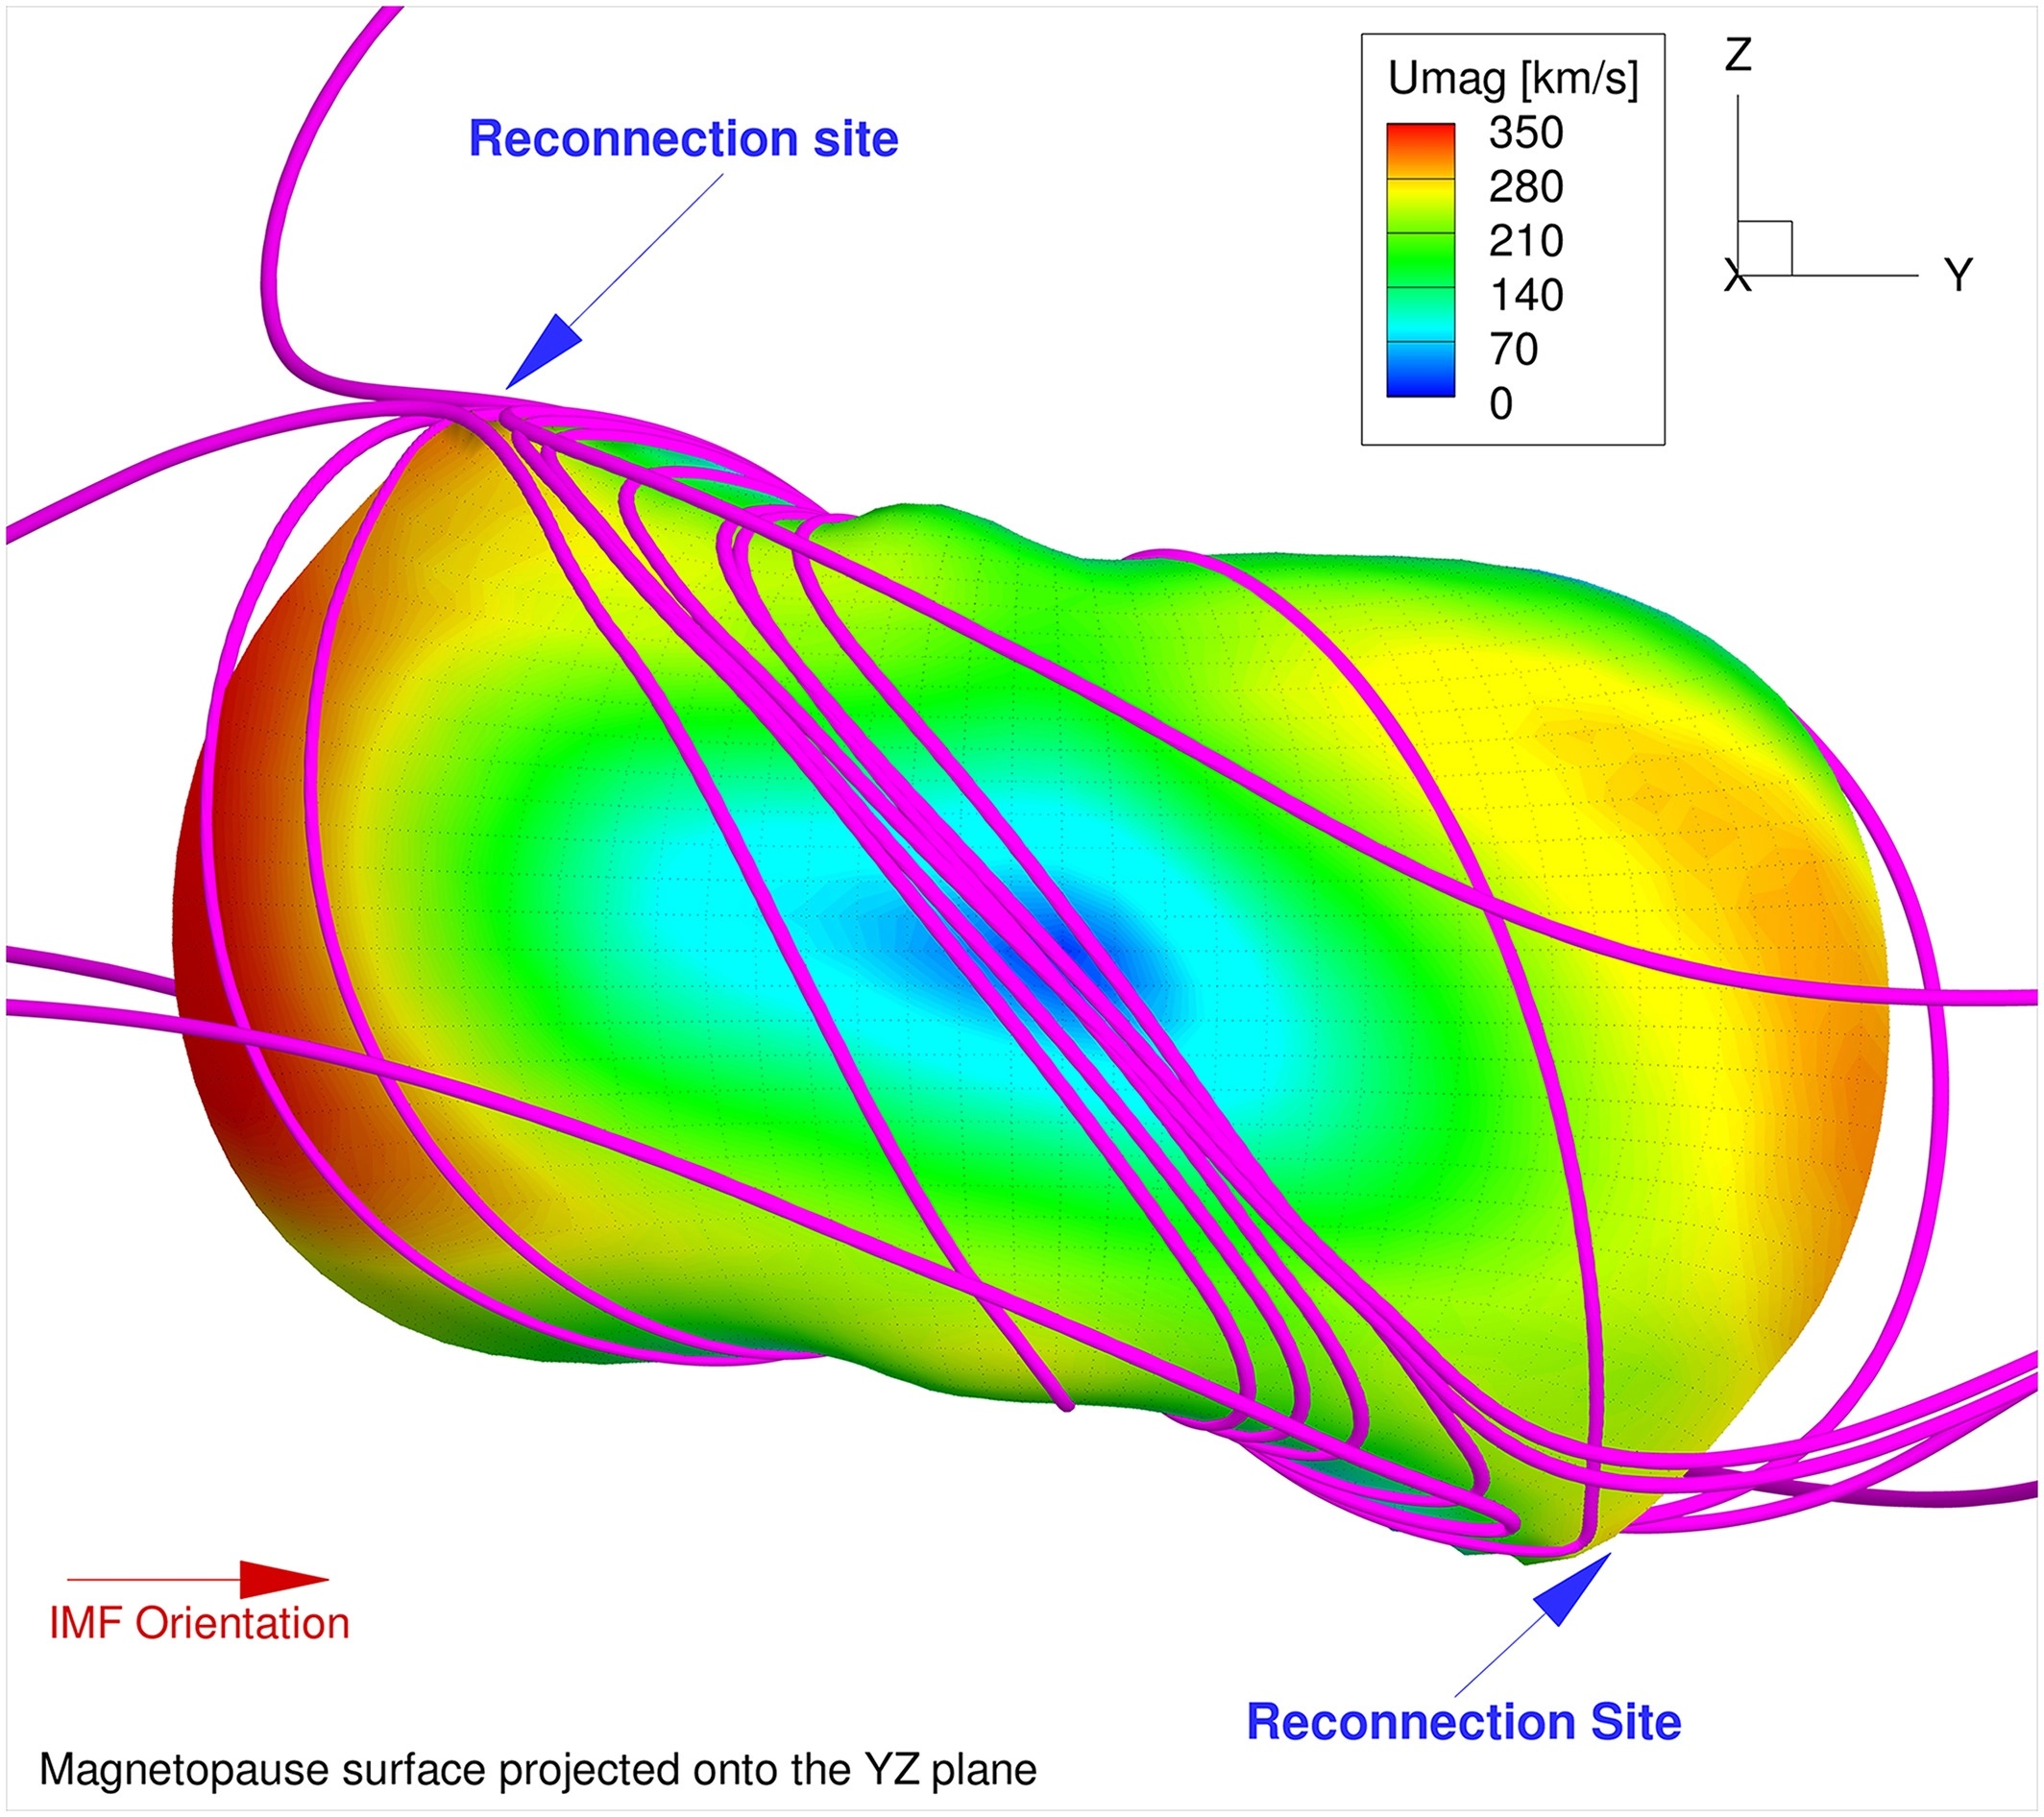
\includegraphics[width=\textwidth]{images4/reconnection-dayside.jpg}
    \caption{The 3D magnetopause surface extracted from our model for the Parker-spiral IMF case. The surface is coloured in contours of plasma speed. Magnetic field lines are shown as magneta tubes. Magnetic reconnection is seen to occur on the mid-latitude dawnside in the northern hemisphere and in the mid-latitude duskside in the southern hemisphere; locations where maximum magnetic shear is expected between the internal field and the IMF.}
    \label{fig:reconnection-dayside}
\end{figure}

For the Parker‐spiral IMF configuration used in our simulation, reconnection is found to occur primarily on the magnetopause at relatively high latitudes (at $\sim50^\circ$) latitude) where the strongest magnetic shear is present. Figure \ref{fig:reconnection-dayside} shows a snapshot of the simulated magnetopause surface extracted from Run 4. The magnetopause surface is determined by identifying the separatrix between magnetospheric and magnetosheath field lines based on 3‐D field line tracing. The color contours on the magnetopause surface represent plasma flow speeds, and sample field lines are superimposed to show the magnetic topology. As shown, under the spiral IMF configuration with positive By, we find that reconnection takes place mainly in two quadrants in the YZ plane: in the northern hemisphere on the dawnside and in the southern hemisphere on the duskside. The reconnection geometry is consistent with the prediction by the analytical model of \cite{Masters2017} for the same IMF configuration.

\subsection{Plasmoid release and variation of open magnetic flux}

In all simulations listed in Table \ref{tab:sw-conditions}, tail reconnection occurs and produces plasmoids. For instance, a large plasmoid can be seen in Figure 6, row 3 in the form of a high‐density region between 00 and 06 LT. After initially being created at a radial distance of $\sim$50–70 $R_J$ on the dawnside, the plasmoid is seen to grow and move tailward, eventually escaping the magnetosphere and lost to the solar wind. In Run 4, a vortex structure is created in the magnetosphere on the duskside at around 40 $R_J$ radial distance from the planet (not shown). The vortex is formed subsequent to a large reconnection event in the magnetotail and it strengthens as it moves sunward, eventually reaching the postnoon sector. The vortex is made of corotating and anticorotating flows and produces a strong ionospheric response in the postnoon sector (Figures 8‐4a and 8‐4b near 16 LT). We believe that this vortex and the subsequent localized bright spot in $J_\parallel$ observed near 16 LT in the ionosphere are due to the interaction of return flow from the duskward tail reconnection site with the corotating magnetospheric plasma and has also previously been observed by \cite{Fukazawa2006a} using their MHD model. 

\begin{figure}
    \centering
    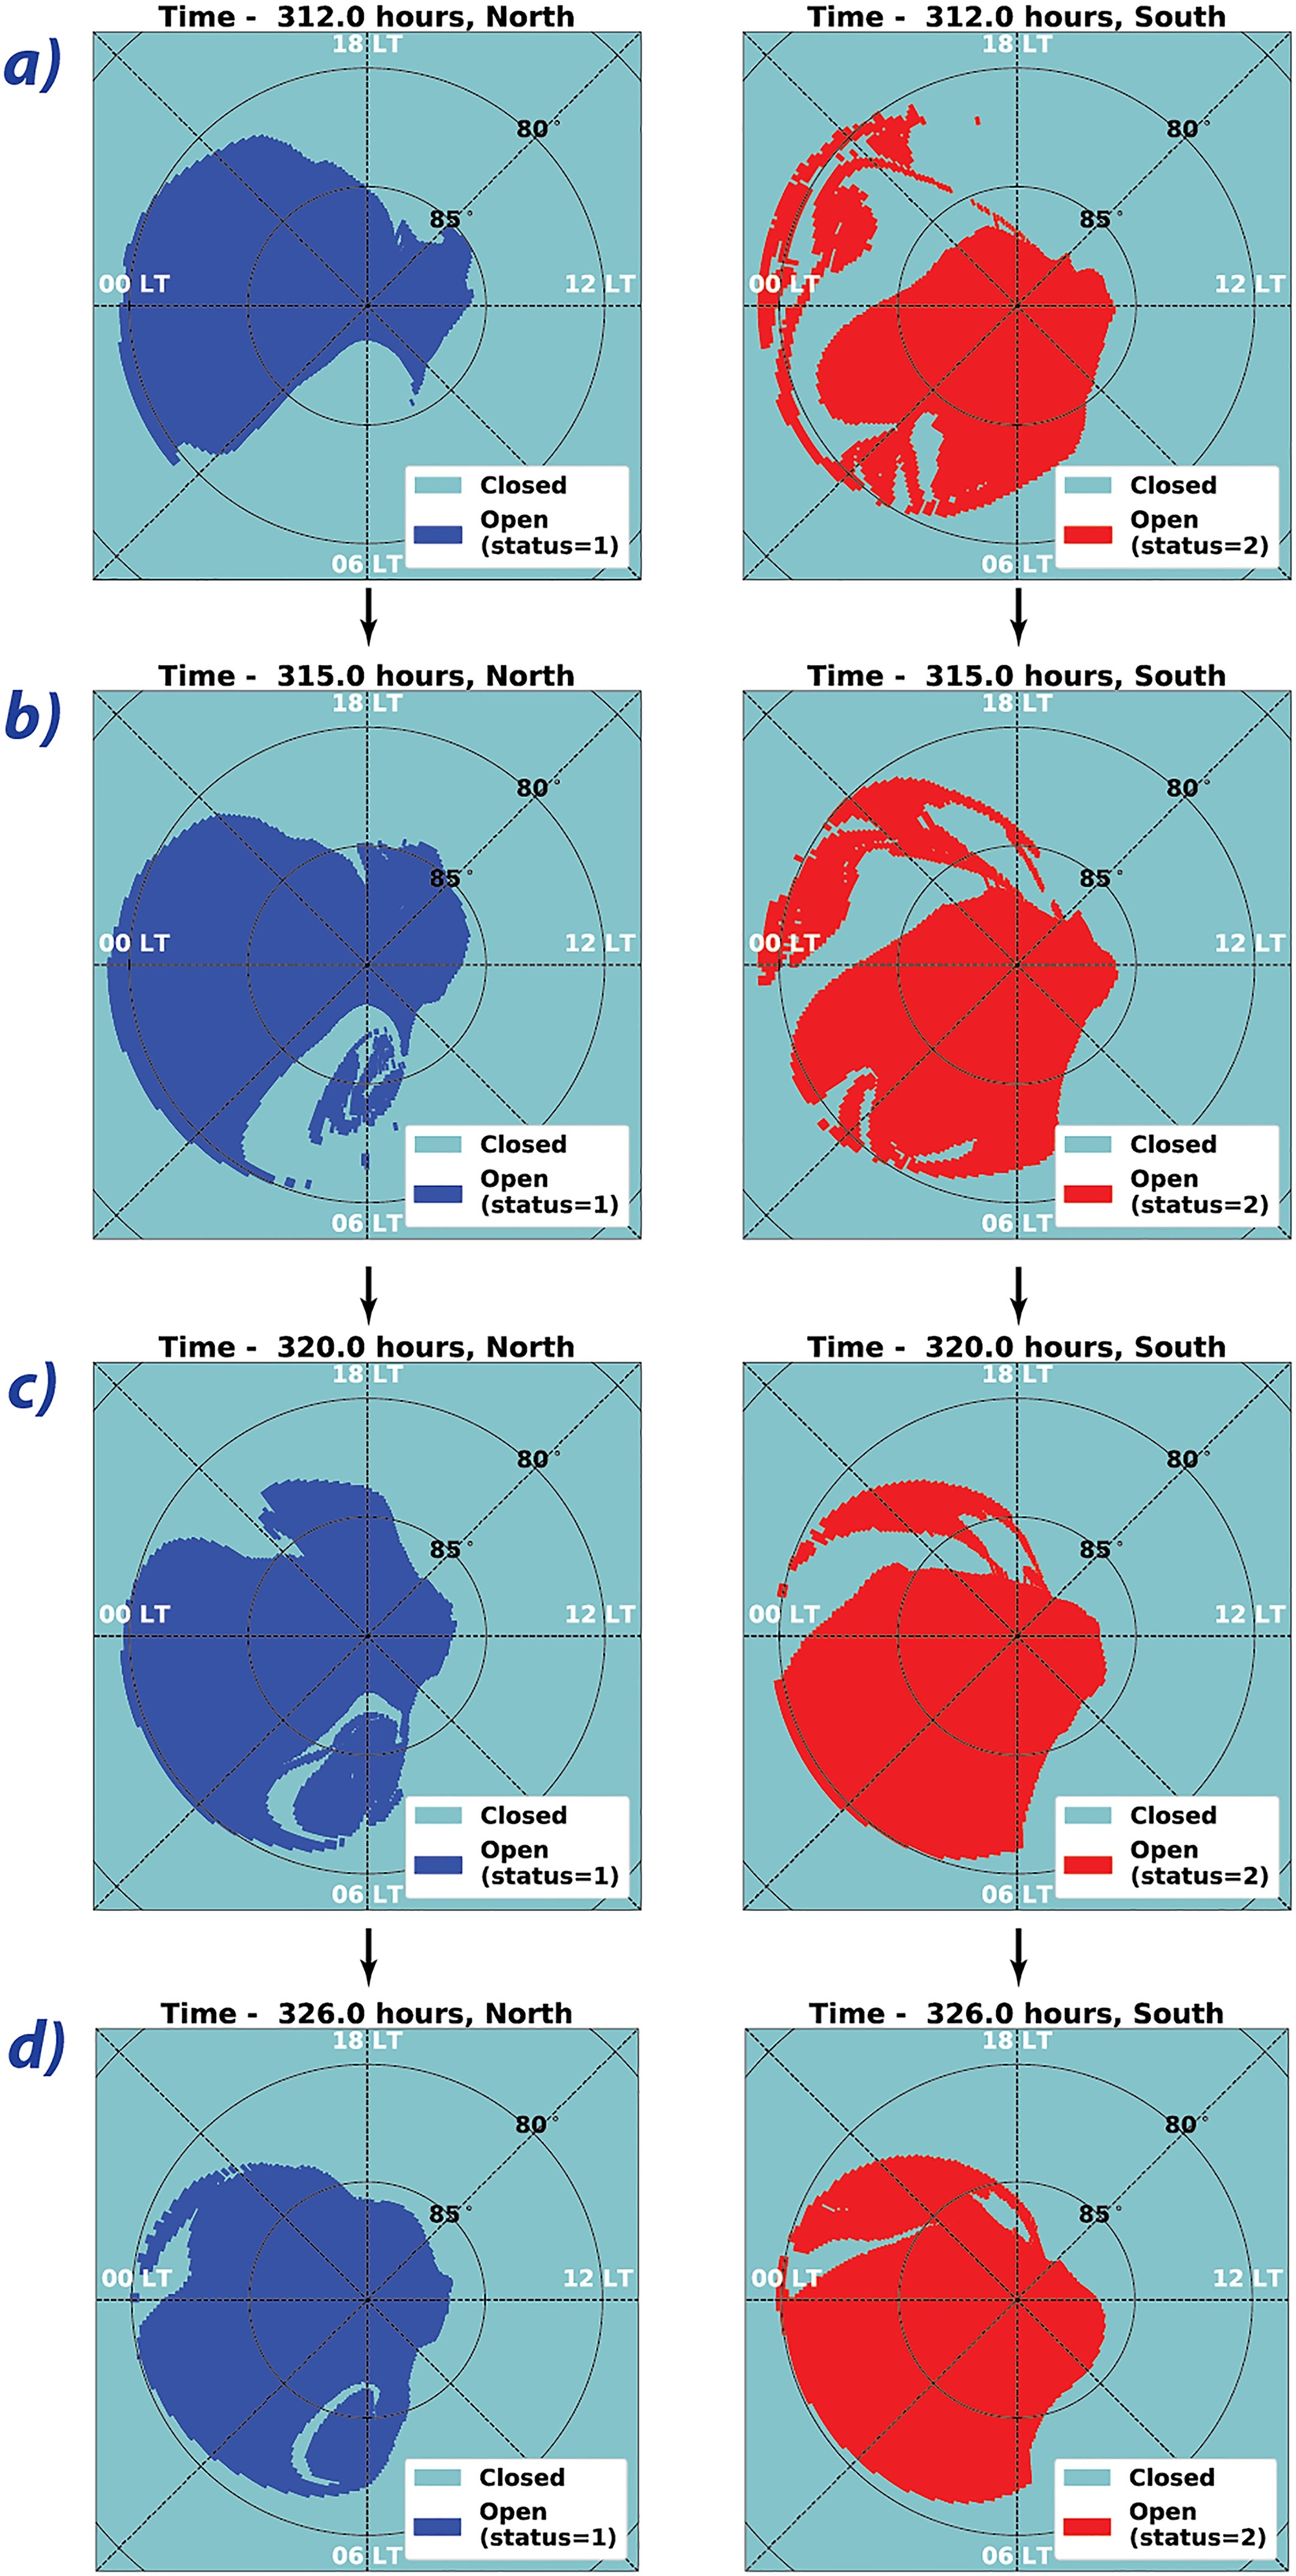
\includegraphics[height=0.9\textheight]{images4/open-flux-variation.jpg}
    \caption{The regions of open flux in the northern and southern regions of the planet ($r=1R_J$) at different times showing the consequence of plasmoid release on magnetic topology. Note the asymmetry between the two hemispheres.}
    \label{fig:open-flux-hemisphere}
\end{figure}

In Figure \ref{fig:ionosphere-currents} the yellow points superimposed onto the contour plots correspond to the OCB identified in our simulations. For each local time and longitudinal position in the ionosphere, we trace 3‐D magnetic field lines from a sphere at 3 $R_J$ to identify any transition between open and closed field lines. If a transition is found, its location on a 1 $R_J$ sphere is determined by using a dipole field line trace, which is then plotted in Figure \ref{fig:open-flux-hemisphere}. Even with $1^\circ$ resolution in both latitude and longitude, our tracing algorithm does not find any such transition during times when the IMF is southward, which is consistent with the picture that the magnetosphere is largely closed under such external conditions. In contrast, under a Parker spiral IMF, the OCB increases in size with time and can reach a latitude of $\sim80^\circ$ on the nightside under strong solar wind driving (column 4). While the size of the OCB tends to vary depending on the upstream conditions, for the various upstream conditions examined in our simulations it is always located poleward (by at least a few degrees) of the main oval of upward field‐aligned currents arising from corotation breakdown, which lies at $\sim75^\circ$ latitude. 

For further analysis we divide the magnetic field lines extracted from our MHD model into four categories, denoted by the “status” variable (Table 2). A status value of 0 represents a closed field line with both ends connected to the planet. A status value of 1 or 2 implies an open field line with one footprint in the northern or southern hemisphere, respectively, while a status value of 3 refers to those field lines with both ends in the solar wind, which we call disconnected field lines. Figure \ref{fig:open-flux-hemisphere} shows the status of field lines seeded from the northern and southern ionosphere, whereas Figure \ref{fig:status-magnetosphere} shows the status of field lines seeded from the equatorial plane in the magnetosphere. 

\subsection{Magnetic topology associated with plasmoid release}

In Figure \ref{fig:open-flux-hemisphere}, we show the status maps of the northern and southern hemispheres on a 1 $R_J$ sphere, at different times during the sequence of a plasmoid release. For both hemispheres, the cyan regions contain field lines that are closed (status = 0). For the northern hemisphere panels, the dark blue regions contain open field lines (status = 1) that magnetically map to the solar wind. For the southern hemisphere panels, the red regions indicate open field lines (status = 2) that map to the solar wind. It is immediately clear from Figure \ref{fig:open-flux-hemisphere} that these status maps are not north‐south symmetric, with stark differences in the topology between the two hemispheres. 

Two plasmoids are observed in the magnetosphere during the times shown in Figure \ref{fig:open-flux-hemisphere}: a relatively small size plasmoid on the duskside and a much larger plasmoid near dawn. When the plasmoids are initially formed, they contain predominantly closed flux. This is consistent with the idea that plasmoids form due to the Vasyliunas cycle are created on closed field lines. As the plasmoids move tailward, they grow in size and create a region of closed flux inside the polar cap. The large plasmoid in the dawn sector of the magnetosphere can be identified by its status signature on the dawnside in the form of a large region of closed flux, whereas the smaller plasmoid in the dusk sector also creates a similar region of closed flux in the duskward polar cap. With time, the plasmoids grow and interact with the surrounding plasma and magnetic field, which creates rather complicated magnetic field structures that contain intertwined open and closed field lines (Figure \ref{fig:open-flux-hemisphere}b). As the plasmoids move further down the magnetotail, they grow in size and the status signatures associated with plasmoids move toward midnight (previously at dawn and dusk) and the high‐latitude region in the ionosphere starts to be filled with open field lines. With time, the ratio of open field lines to closed field lines in the plasmoid footprint increases in both the northern and southern hemispheres. As a result, the tail plasmoids, when mapped magnetically to the ionosphere, correspond to a stripe‐like structure. 

Observations of the polar aurorae of Jupiter show various intriguing features such as arcs and filaments \cite{Grodent2003a,McComas2007,Nichols2009a} that have been suggested to be linked to dynamic processes in the solar wind and magnetotail. Our simulation results show that the polar regions of the planet, which are often assumed to lie on open field lines, may magnetically connect to distant regions in the magnetotail associated with a plasmoid. While our MHD simulation does not directly model the kinetic physics of particle energization associated with reconnection, the magnetic topology associated with plasmoid release and propagation through the tail region as seen in our simulation suggests that energization associated with tail plasmoid release may provide a plausible explanation for the observed arc‐like or filament‐like aurora structures. 

\begin{figure}
    \centering
    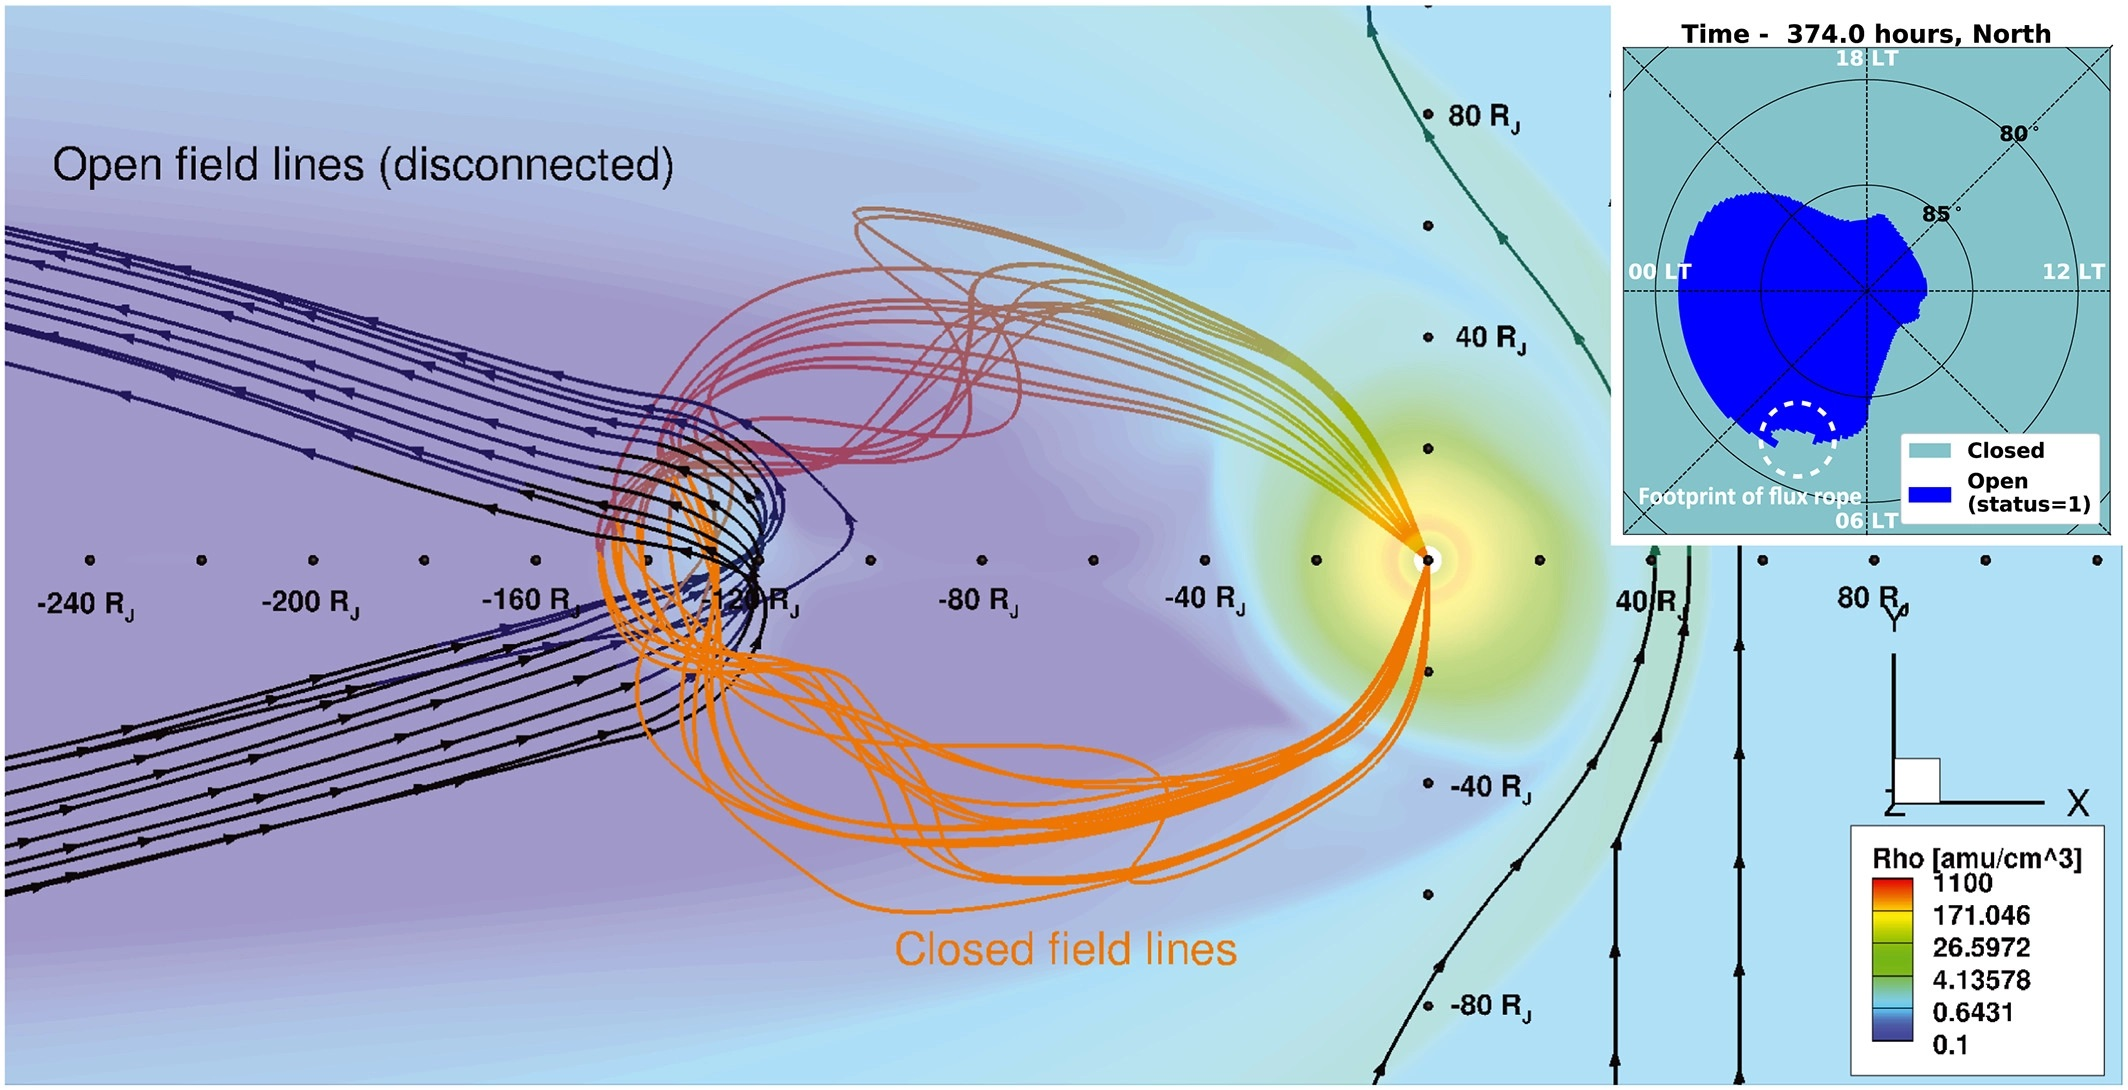
\includegraphics[width=\textwidth]{images4/plasmoid-3d-inset.jpg}
    \caption{3D magnetic field lines threading a plasmoid are shown. Orange field lines are closed, however they are constrained by open field lines which have both ends in the solar wind. The corresponding topology map at this particular simulation time is shown in the inset, where the footprint of the flux rope has been marked.}
    \label{fig:plasmoid-3d-inset}
\end{figure}

In Figure \ref{fig:plasmoid-3d-inset}, we show the three‐dimensional magnetic field lines associated with the tail plasmoid along with the plasma density contours in the equatorial plane. Orange field lines are closed field lines, whereas black field lines are “disconnected” field lines with both ends in the solar wind. It can be seen that although the plasmoid is generated on and still contains closed field lines, it is surrounded by open field lines as it moves tailward. The inset in Figure \ref{fig:plasmoid-3d-inset} shows the corresponding ionospheric status map in a similar format as Figure \ref{fig:open-flux-hemisphere}. Since this plasmoid is noticeably smaller, it has a smaller, but consistent, status signature in the form of a region of closed flux in the polar cap on the nightside. 

\subsection{Open flux in the magnetosphere}

\begin{figure}
    \centering
    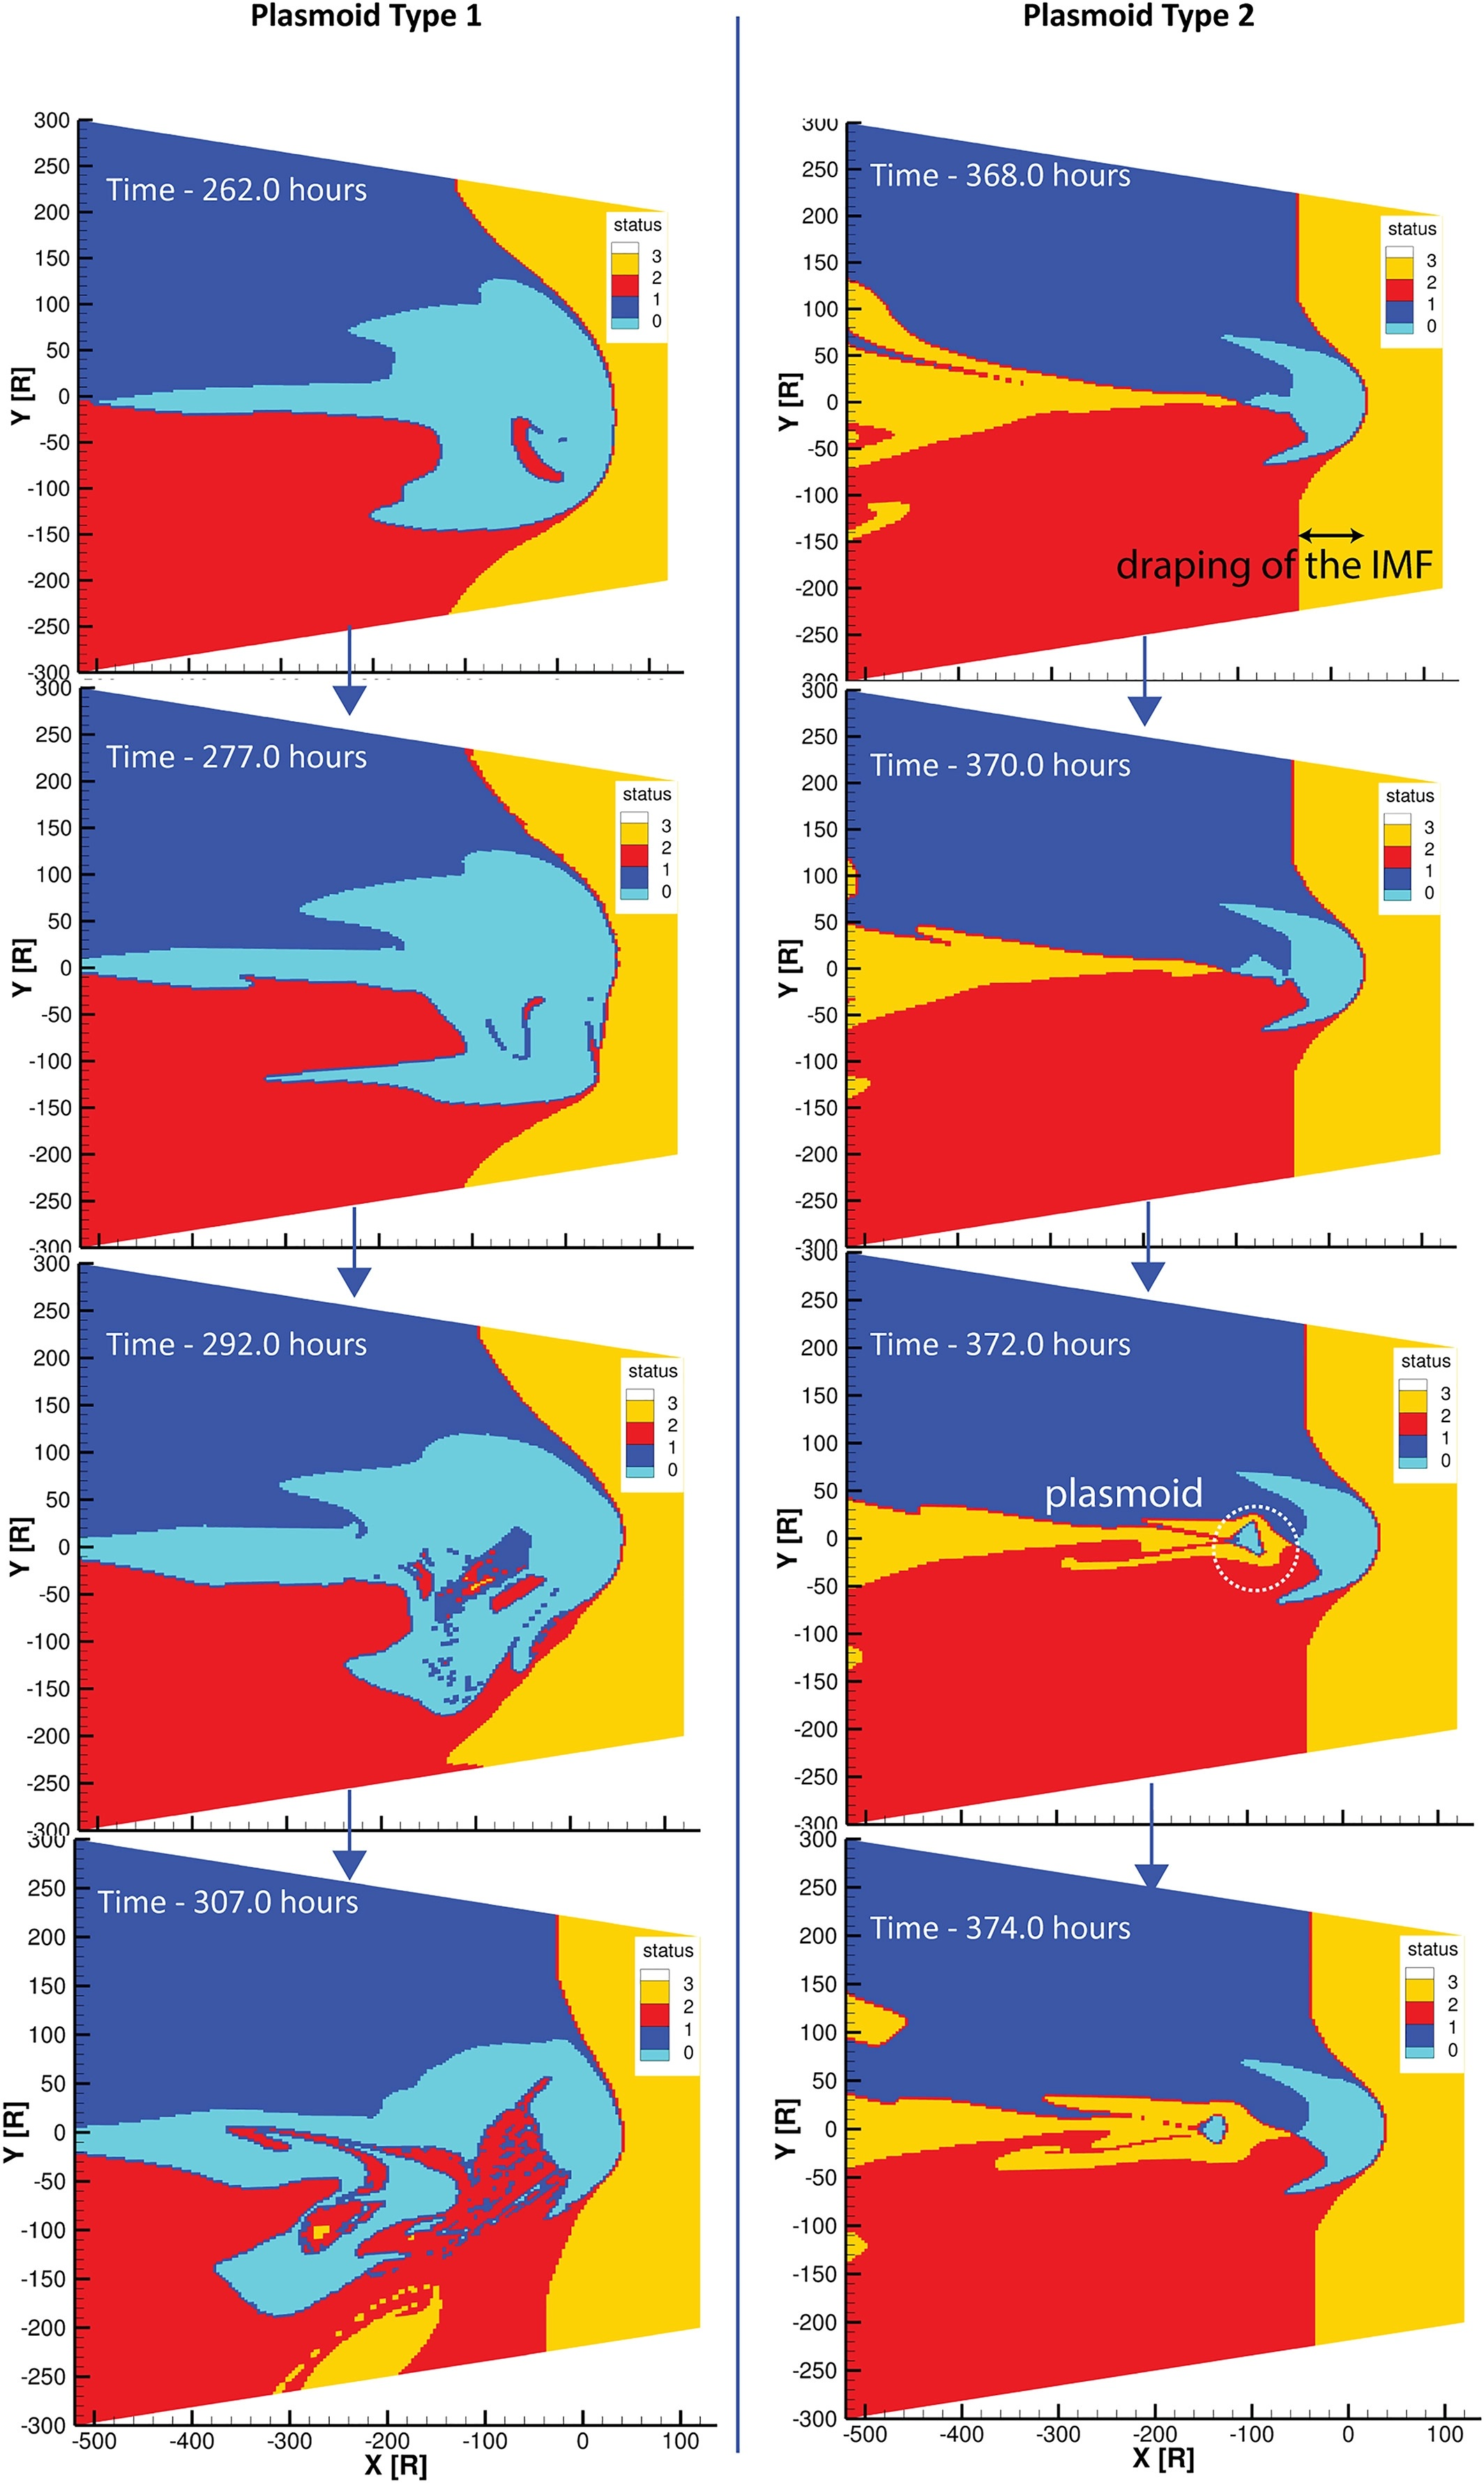
\includegraphics[height=0.8\textheight]{images4/status-fieldlines-magnetosphere.jpg}
    \caption{Topology maps of the magnetosphere during different stages of plasmoid release. On the left are the large Type-1 plasmoids, where the right column shows the progression of a relatively small Type-2 plasmoids. Both plasmoids originate within closed field lines and get surrounded by open field lines as they travel tailward.}
    \label{fig:status-magnetosphere}
\end{figure}

To complement the analysis of the status of field lines shown in section 6.1, we repeated the same procedure of tracing field lines starting in the equatorial plane of the magnetosphere. The corresponding magnetospheric status maps are shown in Figure \ref{fig:status-magnetosphere} for two different types of plasmoids that we will call Type 1 and Type 2, respectively. The left column shows a plasmoid of Type 1, which is a large plasmoid released on the dawnside, whereas the right column shows a plasmoid of Type 2, which is released near midnight. Both plasmoids have some common features, namely, they both originate from closed field lines. After release, the Type 1 plasmoid severely distorts the magnetic topology of the magnetotail. Upon close examination, one can see regions of closed field lines interspersed within large regions of open field lines. The Type 2 plasmoid, on the other hand, has a cleaner topological fallout. After being detached as a “blob” of closed flux, the Type 2 plasmoid is surrounded by disconnected field lines (status = 3, both ends in the solar wind) even though it is located deep inside the magnetosphere. With time, the Type 2 plasmoid moves tailward and the region of closed flux associated with the plasmoid decreases in size. However, the region of disconnected flux in the magnetotail expands after the release of a Type 2 plasmoid. 

Another feature which can be recognized in Figure \ref{fig:status-magnetosphere} is the stark separation between dayside disconnected field lines and the open (status = 1 and 2) field lines on the dawn and dusk flanks, as can be identified through the vertical demarcation at $x = -40 R_J$ in column 2. We traced 3‐D magnetic field lines which suggest that this vertical demarcation is linked to the draping of the IMF around the magnetopause. That field lines in the magnetosheath drape around the magnetopause has been discussed in detail for Earth and Saturn \cite{Crooker1985,Sulaiman2014,Sulaiman2017Large-scaleMagnetosphere} and is expected to be more pronounced at Jupiter due to the large polar flattening of the magnetosphere \cite{Erkaev1996,Farrugia1998,Slavin1985}. While our model does predict the draping of the IMF around Jupiter's magnetopause, the degree of polar flattening in our model is lower than previous predictions ($\epsilon=\sim$0.3, expected to be $\sim$0.8 according to \citeNP{Slavin1985}). 

\subsection{Rate of change of open flux in the magnetosphere}

\begin{figure}
    \centering
    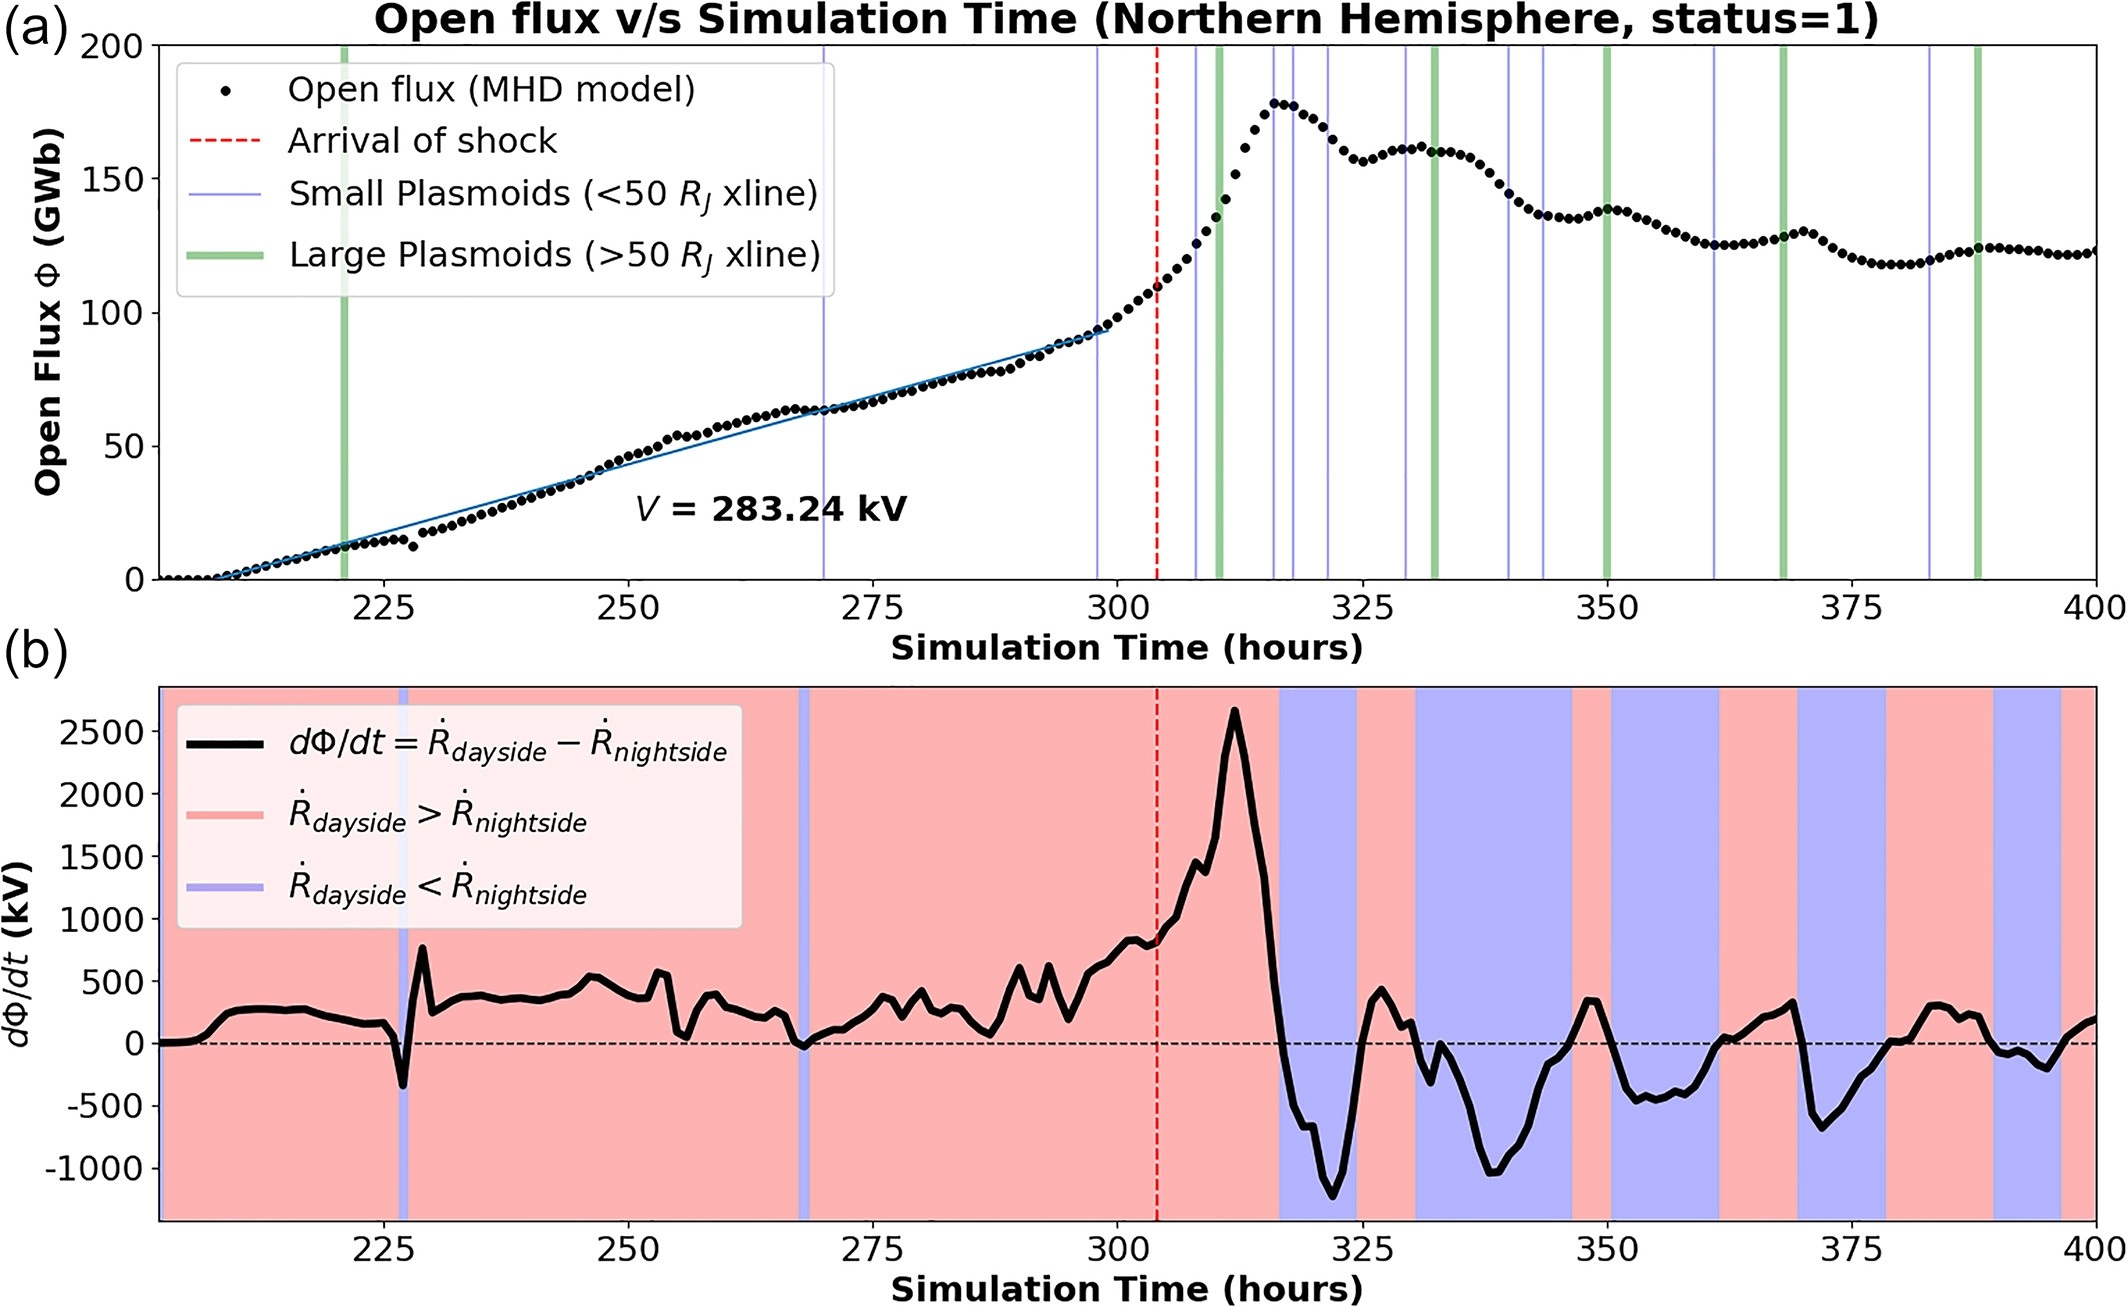
\includegraphics[width=\textwidth]{images4/open-flux-time.jpg}
    \caption{Variation of open flux in the MHD simulation, along with the rate of change. Periods of positive rate of change of flux indicate times when dayside reconnection is dominant, whereas those with negative change indicate times when nightside reconnection is active. Alternating periods of negative and positive change signify repetitive plasmoid release.}
    \label{fig:open-flux-time}
\end{figure}

After identifying the status of each point on the 1 $R_J$ sphere for multiple times in our simulations, we integrate the open magnetic flux within the open field region in the northern hemisphere of the planet. Figure \ref{fig:open-flux-time}a shows the variation of this calculated open flux in our model as a function of simulation time for Parker‐spiral IMF (purely $B_Y$) but different solar wind dynamic pressures. The black points show the open flux calculated in our simulation, while the dashed red vertical line marks the time when the introduced forward shock arrives at the bow shock. To reveal potential correlation between plasmoid release and open flux variations, we overlay solid lines in this figure to mark the times when plasmoid release occurs in the simulation. We identify plasmoids in the model based mainly on the $B_Z$ component (the normal component to the tail current sheet). A bipolar variation of $B_Z$ in the equatorial plane is an indication that a reconnection event has occurred in the magnetotail. Typically, plasmoids generated in our model tend to grow in size as they move tailward. Therefore, we further divide the identified plasmoids into two groups based on their maximum size in the cross‐tail direction ($Y$ direction): large plasmoids which have a cross‐tail width larger than 50 $R_J$ at their maximum extent and small plasmoids whose maximum width is $<50 R_J$. Green thick lines and thin blue lines represent the times when large and small plasmoids are released, respectively.

Prior to the shock arrival at $t = 302$ hr, the IMF along with the solar wind parameters remain fixed. During this interval, the open flux in our model gradually builds up due to the magnetopause reconnection. At around $t = 223$ hr (marked by the solid green vertical line), a relatively large plasmoid with a cross‐tail width exceeding 50 $R_J$ forms in the magnetotail that closes some of the open flux stored in the tail lobes, which can be seen as the change of slope in the time history of the open flux. During this period, there are also a couple of smaller‐scale plasmoids (with cross‐tail width $<50 R_J$) formed, as marked by the solid blue vertical lines in Figure \ref{fig:open-flux-hemisphere}. After the shock arrival at $t = 302$ hr, the rate at which the open flux is added to the polar cap increases due to the enhanced solar wind convectional electric field associated with the shock. About 25 hr after the shock impact, a large‐size plasmoid is formed and released in the tail that results in a significant reduction of the open flux. After the impingement of the shock, the compressed magnetosphere experiences frequent plasmoid release, both large and small. Compared to the situation seen in the simulation during the nominal solar wind conditions where plasmoid release occurs every 20 to 50 hr, the occurrence rate is significantly higher in the compressed case, which is of the order of one plasmoid every few hours. A similar behavior has been seen in the MHD model of Saturn by \cite{Jia2012} who found more frequent plasmoid releases during periods of stronger solar wind driving. 

The time variation of the open flux provides a useful measure of how the magnetosphere responds globally to the solar wind driving and internal dynamics. As discussed above, dayside reconnection would add open flux to the polar cap whereas tail reconnection would potentially close open flux stored in the tail lobes. Therefore, the time rate of change of the open flux can be used to quantify the global reconnection efficiency, which depends on the difference in the reconnection rates between the dayside magnetopause reconnection and the tail reconnection. At the beginning of the simulation, in the absence of tail reconnection, we find that the open flux increases at a rate of $\sim$284 kV, which corresponds approximately to the global reconnection rate under the solar wind conditions listed in Table \ref{tab:sw-conditions}, column 2.

In Figure \ref{fig:open-flux-time}b, we show the calculated rate of change of open flux in the northern hemisphere (status = 1), that is, $d\Phi/dt$ as a function of simulation time. After the shock is introduced in the simulation, the rate of increase of open flux increases, corresponding to a peak global reconnection potential of $\sim$2 MV. This increase in the reconnection rate on the dayside is primarily due to enhanced solar wind speed and increased IMF strength due to compression and hence the convectional electric field behind the shock. At later times, the open flux in our simulation is found to decrease and increase periodically at a period of $\sim$20 hr, highlighting the competing influence of magnetopause reconnection (which serves to open magnetic flux) and nightside reconnection (which decreases the net open magnetic flux). Closer examination reveals that the decreases in open flux are also correlated with the release of large plasmoids. \citeA{Walker2016} report on simulations of the Jovian magnetosphere performed by \citeA{Fukazawa2006a} and also found quasi‐periodic increase and decrease in open flux with a similar period of $\sim$20–30 hr. 

In discussing Figure \ref{fig:open-flux-hemisphere} we noted that the release of plasmoids creates a region of open flux in the polar cap, which may seem contradictory to these findings. However, it must also be noted that the overall size of the polar cap also depends on many other factors, such as the difference between reconnection rate on the dayside versus the nightside. Figure \ref{fig:status-magnetosphere} clearly demonstrates that plasmoid release increases the amount of disconnected flux in the magnetosphere. Since the disconnected field lines, by definition, cannot magnetically map to the northern hemisphere, they are not accounted for in our calculation for net open flux which is done on a 1 $R_J$ sphere for Jupiter (thereby only considering status = 1 type field lines). Figure \ref{fig:status-magnetosphere} also shows that with the increase of disconnected flux in the magnetotail, the amount of connected open flux (i.e., status = 1 and 2) decreases. This would decrease the overall size of the polar cap, which would lead to decreased status = 1 flux. The overall shrinking of the polar cap can also be seen in Figure \ref{fig:open-flux-hemisphere}. 

As time progresses the dayside and nightside reconnection rates seem to approach steady state, which can be seen in Figure \ref{fig:open-flux-time}b where fluctuations in $d\Phi/dt$ decrease with time. For the compressed magnetosphere, at the end of our simulation ($t = 400$ hr) the total open flux amounts to $\sim$ 120 GWb. It is interesting to note that the creation of open flux is largely due to the reconnection on the magnetopause, and the result that the net open flux seems to reach a steady state implies that flux closure on the nightside or elsewhere is happening in a manner expected by the terrestrial‐like Dungey cycle. Although we have not yet identified any preferential spatial location where flux closure is consistently occurring, it is clear that both Vasyliunas cycle reconnection (detachment of plasmoids on closed field lines) and Dungey cycle‐type flux closure contribute to the circulation of magnetic flux in Jupiter's magnetosphere. 

Plasmoids generated in Jupiter's magnetotail may be a result of a near‐planet like flux closure event attributed to the Dungey cycle or a result of centrifugal stresses exerted on the corotating plasma, that is, the Vasyliunas cycle, both of which may cause reconnection onset on closed field lines. When the IMF is southward (Run 1), absence of dayside magnetopause reconnection would essentially shut off the Dungey cycle. However, plasmoids are still observed in this case (not shown), and they are a direct product of the Vasyliunas cycle. In this case the plasmoid, once generated, is constrained by the surrounding closed field lines, and “escapes” through the magnetopause. In contrast, when the IMF is in the Parker‐spiral configuration, dayside magnetopause reconnection would add open field to the tail lobes. In this scenario, plasmoids generated due to a tail reconnection event may induce closure of open flux in the tail lobes \cite{Cowley2008} regardless of the original cause of reconnection onset. The lobe reconnection‐produced field lines, which are carried by fast‐moving reconnection jets moving behind the plasmoids, would facilitate the escape of plasmoids down tail. These findings from our Jupiter simulations are similar to those reported for global simulations of Saturn's magnetosphere \cite{Jia2012}. 

As noted earlier, the global simulation presented here is based on an ideal MHD model, in which no kinetic physics is included to describe reconnection. However, reconnection does occur in MHD simulations, which is facilitated by numerical resistivity. It is interesting to compare the global reconnection rate and the resultant amount of open flux in our MHD model with prior estimates based on observations and analytical models. For instance, \citeA{Masters2017} presented an analytical method to estimate the total reconnection potential at Jupiter's magnetopause under different solar wind conditions, and he predicted a dayside reconnection potential ranging between 200 and 1,000 kV. The reconnection potentials estimated in our simulations are in general agreement with the Masters model results. Further, based on auroral observations and magnetic field modeling, \citeA{Nichols2006Magnetopause5AU,Vogt2011a} estimated the typical amount of open flux present in Jupiter's magnetosphere, and their results give a range of 300–700 GWb. The maximum amount of open flux seen in our simulations is about 175 GWb, which is slightly lower than previous estimates and could be related to our use of an ideal axisymmetric dipole for the planetary magnetic field.

\section{Summary}

Our simulations show that magnetic reconnection on the dayside magnetopause at Jupiter creates open flux in the polar caps. The open field lines are magnetically connected to the polar regions of the planet and occupy a relatively small area poleward of the main auroral oval. 

Plasmoid release in the tail has long been suggested to be an important means of plasma transport, and signatures of plasmoids have indeed been found in various in situ observations in Jupiter's magnetotail. Our global simulations also show plasmoid formation and release due to reconnection in the magnetotail. The majority of plasmoids seen in our simulations appear to form initially on closed magnetic field lines, consistent with the picture proposed by \citeA{Vasyliunas1983a}. While differing in size, all the plasmoids produced in the simulations develop a complex magnetic topology as they evolve and propagate downtail. As an example, we have shown the time evolution of two plasmoids with different sizes and their mapping to the polar ionosphere. Our magnetic mapping results support the previous hypothesis that the complex morphology of tail plasmoids may be responsible for creating puzzling auroral features such as arcs and filaments \cite{Grodent2003a,McComas2007,Nichols2009a}. 

As a quantitative measure of the influence of the external driver on the global magnetospheric configuration, we have identified the OCB throughout our simulations by tracing 3D magnetic field lines. We have also calculated the total amount of open flux within the magnetosphere and examine the time evolution of the open flux in response to the changes imposed on the upstream parameters. For southward IMF, the magnetosphere has little to no open flux, as expected. As the IMF orientation is changed to a more realistic Parker spiral configuration, open magnetic flux starts to be added to the magnetosphere due to the dayside magnetopause reconnection and as such the OCB in the ionosphere starts to expand in size moving equatorward. In all the simulations present here, the OCB is found to be always located poleward by at least a few degrees of the main oval of upward field‐aligned currents associated with corotation breakdown. The total amount of open flux is found to peak around 200 GWb for typical Parker‐spiral IMF conditions, which is about a factor of 2 smaller than previously published estimates \cite{Vogt2011a}. There is a clear correlation between the reduction of open flux and the release of plasmoids in the tail, whose occurrence frequency appears to be affected by the solar wind convectional electric field with more frequent release under stronger driving. Based on the time rate of change of the open magnetic flux, we estimate the average potential drop associated with the dayside reconnection under nominal solar wind conditions to be approximately 280 kV, which is about a factor of 2 lower than previous estimates \cite{Masters2017}. 

Our simulations also show that the frequency at which plasmoids are released in the magnetotail increases due to higher solar wind dynamic pressure, and are more frequently observed in a situation when the magnetosphere contains open field lines. These results support the hypothesis that the Dungey cycle reconnection occurs in the Jovian magnetotail, but it is not limited to certain regions in the exterior of the magnetosphere and can occur as a result of the internally driven Vasyliunas cycle reconnection, if the field lines which constrain the plasmoids are open to the interplanetary magnetic field. In such cases, plasmoid release induces reconnection in the tail lobe field diffusing toward the Vasyliunas X-line, thus accomplishing flux closure. 
